% !TeX root = ../tfg.tex
% !TeX encoding = utf8
%
%*******************************************************
% Introducción
%*******************************************************

% \manualmark
%\markboth{\textsc{Introducción}}{\textsc{Introducción}} 

\chapter{Introducción}

En el contexto de la actual revolución tecnológica, diversas arquitecturas de redes neuronales han demostrado ser especialmente eficaces en tareas complejas del ámbito del aprendizaje profundo. Modelos como las redes convolucionales, los Transformers y los modelos de difusión han mostrado un rendimiento notable en campos como la visión por computador, el procesamiento del lenguaje natural y la generación de contenido, debido a su gran capacidad para analizar grandes volúmenes de datos. En este trabajo, nos centraremos en las redes neuronales convolucionales, dada su consolidada capacidad para extraer representaciones significativas de la información visual, logrando en muchos casos superar el rendimiento alcanzado por los humanos en tareas de clasificación y detección de imágenes.

En los últimos años y bajo este marco de expansión y evolución del aprendizaje, el \emph{Deep Double Descent} ha surgido como un importante campo de interés dentro de este ámbito, desafíando los principios clásicos del aprendizaje estadístico. La sabiduría tradicional sugiere que, a medida que aumenta la complejidad del modelo, el error fuera de la muestra disminuye hasta alcanzar un mínimo para, a continuación, aumentar debido al sobreajuste (formando la tradicional curva con forma de ``U'').

Este concepto, conocido como equilibrio entre sesgo y varianza, difiere de las recientes observaciones obtenidas, especialmente en modelos de aprendizaje profundo, en los que puede producirse una segunda disminución del error fuera de la muestra, alcanzando un nuevo mínimo y formando una nueva gráfica del error de generalización que presenta dos descensos. Este novedoso hecho pone en tela de juicio la sabiduría clásica sobre el tema y proporciona nuevas perspectivas a la hora de crear y entrenar los modelos.

Como consecuencia, este Trabajo de Fin de Grado (TFG) se ocupa de explorar el concepto de \emph{Deep Double Descent}, sus fundamentos teóricos y sus implicaciones para el aprendizaje automático moderno. Un área clave de interés es cómo este fenómeno se manifiesta en redes neuronales profundas, conocidas por su enorme complejidad en cuanto a número de párametros se refiere y su potencial de sobreajuste. A pesar de que los modelos de aprendizaje profundo han tenido gran éxito en diversas aplicaciones, como la visión por computador o el procesamiento de lenguaje natural, la curva del doble descenso aporta nuevo conocimiento sobre cómo estos modelos pueden llegar a generalizar en un régimen que ha sido vagamente estudiado y explorado: el régimen sobreparametrizado. La idea clave es la existencia de dos zonas de actuación del modelo claramente diferenciadas, la zona infraparametrizada y la zona sobreparametrizada. Sin embargo, formalizar esta idea no es trivial, dado que los modelos profundos funcionan como «cajas negras», lo que hace que, a medida que aumenta su complejidad, resulte cada vez más difícil interpretar y analizar su funcionamiento interno.

Aunque cada vez hay más estudios abordando este hecho, muchos de ellos se centran en una perspectiva empírica del mismo, sin ofrecer una base teórica suficiente, mientras que otros sistematizan conceptos sin llegar a conclusiones prácticas. En este TFG, y con el objetivo de ofrecer una comprensión lo más completa posible, buscamos cerrar la brecha entre la teoría y la práctica, unificando explicaciones teóricas suficientemente rigurosas con ejemplos empíricos del mundo real.


\section{Definición del problema}

\begin{figure}[h]
    \centering
    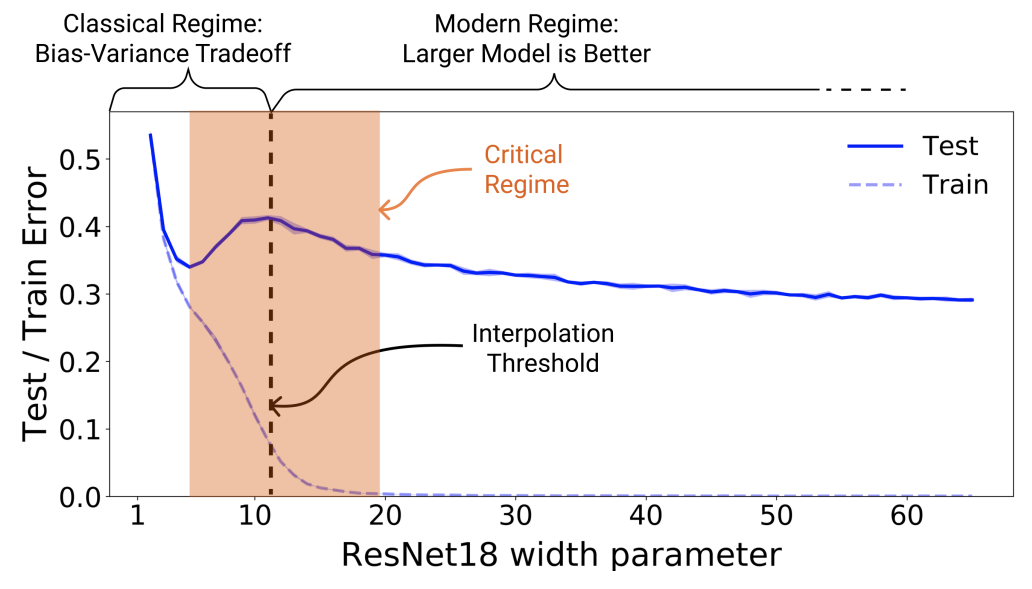
\includegraphics[width=0.9\textwidth]{img/problem-definition.png}
    \caption[Ejemplo de doble descenso profundo en ResNet$18$~\cite{Nakkiran2019}.] {Ejemplo de doble descenso en ResNet18~\cite{Nakkiran2019}. La imagen muestra el error de entrenamiento (\textit{train error}, curva discontinua) y de generalización (\textit{test error}, curva continua) para la arquitectura ResNet$18$ con diferente capacidad (número de parámetros). En ella, observamos las tres regiones de actuación del modelo, así como el máximo del error de generalización correspondiente al umbral de interpolación y los dos descensos de dicho error.}\label{fig:ejemplo-definicion-double-descent}
\end{figure}

El término \textbf{doble descenso profundo} \emph{(Deep Double Descent~\cite{Belkin2019})} describe la forma que toma la curva del error de generalización (error fuera de la muestra, \textit{out-of-sample error}) de un modelo de aprendizaje como función de la capacidad del mismo. De manera intuitiva, podemos distinguir tres zonas o regiones diferenciadas en dicha curva:

\begin{itemize}
    \item \textbf{Región clásica (infraparametrizada):} En esta región, el modelo no puede capturar toda la complejidad subyacente de la distribución de los datos debido a su baja capacidad. Como resultado, el error de generalización disminuirá inicialmente, ligado al hecho de que el modelo aprende de los datos de entrenamiento. Sin embargo, llegado un momento, el error de generalización aumentará de manera progresiva (véase Figura~\ref{fig:ejemplo-definicion-double-descent}, parte de la figura etiquetada como ``Classical Regime: Bias-Variance Tradeoff'') dando lugar a la clásica curva en forma de ``U'', relacionado con el hecho de que el modelo, en lugar de aprender patrones, memoriza los datos de entrenamiento.

    \item \textbf{Región moderna (sobreparametrizada):} En esta zona, representada en la Figura~\ref{fig:ejemplo-definicion-double-descent} bajo la etiqueta ``Modern Regime: Larger Model is Better'', el modelo tiene una capacidad mayor de la necesaria para ajustar los datos de entrenamiento, es decir, dispone de suficientes herramientas (parámetros) para ajustar cada uno de los datos de entrenamiento. Contrariamente a lo que se esperaría según la sabiduría convencional, el error de generalización no necesariamente aumenta en este región y, bajo ciertas condiciones, dicho error puede reducirse nuevamente, produciendo un nuevo descenso de la curva del error de generalización que se conoce como \emph{doble descenso}.
    
    \item \textbf{Región crítica:} Esta región, indicada en la Figura~\ref{fig:ejemplo-definicion-double-descent} como ``Critical Regime'', marca la transición entre la región infraparametrizada y la región sobreparametrizada y engloba zonas de ambas regiones. Dentro de ella, se encuentra el llamado umbral de interpolación o \textit{interpolation threshold}, que corresponde al punto donde el modelo tiene justo la capacidad suficiente para ajustar de manera prácticamente perfecta los datos de entrenamiento. En este punto crítico, el error de generalización alcanzará su máximo.
       
\end{itemize}

Este doble descenso puede llegar a suponer la obtención de modelos cuyas predicciones sean aún mejores. Sin embargo, se abre la puerta a la investigación del por qué ocurre este novedoso fenómeno, además de tener que replantearnos algunas respuestas, asumidas tradicionalmente como correctas, ante preguntas clásicas del aprendizaje profundo.

\section{Motivación}

En el ámbito del aprendizaje automático, existe una brecha entre el desarrollo empírico y la fundamentación teórica subyacente. Los modelos modernos, en particular las redes neuronales profundas, han demostrado resultados sorprendentes~\cite{Sejnowski2020TheUE, He2020RecentAI} desde la generación de imágenes realistas mediante redes generativas~\cite{Elasri2022, Ruthotto2021} hasta el procesamiento de lenguaje natural (\textit{Natural Language Processing, NLP})~\cite{Kamath2019, Lauriola2022}. Sin embargo, estos resultados se logran sin una adecuada comprensión teórica~\cite{Ben-David2009, Grohs2022}.

Esta capacidad para obtener resultados que consideramos satisfactorios ha llevado a un enfoque predominantemente práctico, donde los avances se suelen producir de manera más rápida a través del ensayo y error y no tanto a través de modelos matemáticos bien fundamentados, lo que impide comprender, desde una perspectiva teórica, tanto la eficacia como las verdaderas limitaciones de estos modelos. El doble descenso plantea cuestiones sobre la sostenibilidad de este enfoque práctico y la necesidad de desarrollar un marco teórico que permita anticipar y guiar estos avances en lugar de simplemente reaccionar ante ellos.

Aunque existen elogiosos esfuerzos para comprender las bases teóricas del deep learning~\cite{Zhang2021,Mallat2016, Prince2023, Bishop2023, Grohs2022, Balestriero2018, Michael2018}, la desconexión entre avances teóricos y prácticos continúa siendo notable. Por ello, en los últimos años han ido apareciendo discrepancias, y se han observado fenómenos de carácter práctico, que han desafiado el conocimiento teórico tradicional. Es aquí donde se enmarca el concepto de \emph{Deep Double Descent}.

De igual manera, este proyecto tiene una relevancia crucial, ya que podría transformar la forma en que se diseñan y optimizan los modelos profundos. Tradicionalmente, el enfoque clásico sugiere que, a medida que se aumenta la complejidad del modelo, este tiende a sobreajustarse a los datos, lo que limita su capacidad de generalización frente a nuevos datos no vistos y motivaba a optar por modelos más simples o incorporar estrategias de regularización. Sin embargo, con la aparición del \textit{Deep Double Descent}, se ha demostrado que, más allá del sobreajuste, los modelos no solo proporcionan mejores predicciones, sino que incluso alcanzan niveles de generalización superiores a los iniciales. Este descubrimiento sugiere que, siguiendo este enfoque, podríamos prescindir de la teoría clásica y centrarnos en desarrollar modelos más complejos. No obstante, las limitaciones computacionales y energéticas siguen representando un desafío en el entrenamiento de grandes modelos de deep learning~\cite{Thompson2022, Cottier2025, Desislavov2023, Strubell2020}. Por ello, en la actualidad, aún se aplican técnicas de regularización para mitigar el sobreajuste y optimizar el uso de recursos.

En conclusión, el \emph{Deep Double Descent} representa un cambio de paradigma, digno de estudio, en el aprendizaje automático. Comprender los principios subyacentes permitiría avanzar en nuestra comprensión teórica del aprendizaje automático, reduciendo la brecha teórico-práctica, e incluso podría contribuir a guiar el diseño y optimización de modelos prácticos más efectivos.

\section{Objetivos}

Los primeros indicios del \textit{Deep Double Descent} se remontan a la década de $1990$ y principios de los años $2000$~\cite{Vallet1989, Opper2001}, aunque no se utilizaba específicamente esa terminología. Estos estudios mostraban la relación entre la complejidad del modelo y el error de generalización, indicando que, en algunos casos, aumentar la complejidad del modelo más allá de cierto punto no incrementaba necesariamente el error de generalización. No obstante, no es hasta $2019$ cuando Belkin et al.~\cite{Belkin2019} abordan la primera investigación formal sobre este tema y le asignan su particular nombre. A partir de ese momento, la comunidad científica comienza a mostrar un creciente interés hasta el día de hoy, lo que nos lleva a catalogarlo como un acontecimiento novedoso.

Por tanto, el objetivo principal de este TFG radica en tratar de \textbf{ofrecer una explicación detallada y estructurada del reciente concepto del \emph{Deep Double Descent}}. Este estudio se centrará en proporcionar una visión actualizada y rigurosa de sus fundamentos teóricos, implicaciones prácticas y relevancia en el desarrollo de modelos modernos, asegurando que el contenido se mantenga en concordancia con los avances más recientes en la investigación. Para alcanzar este objetivo, se han definido dos líneas de trabajo profundamente interrelacionadas: una orientada al desarrollo \textbf{matemático} y otra enfocada a la parte \textbf{informática}. Ambas se desarrollan de manera conjunta y complementaria, de modo que los avances teóricos guían la implementación práctica, mientras que los resultados experimentales permiten validar y enriquecer la comprensión teórica. A su vez, cada línea de trabajo se descompone en una serie de objetivos parciales que, en conjunto, dirigen el desarrollo del proyecto.

\subsection{Objetivo matemático}

El objetivo fundamental para la parte matemática consiste en profundizar en la comprensión teórica del \textit{Deep Double Descent} a través del estudio detallado de sus fundamentos matemáticos, explorando las relaciones con conceptos clásicos como el equilibrio sesgo-varianza y su posible conexión con la teoría de la aproximación no lineal. Con el fin de abordar de forma sistemática las distintas fases de este análisis, el presente objetivo se descompondrá en los siguientes objetivos parciales:

\begin{itemize}
    \item Realizar un análisis exhaustivo y detallado del estado del arte, revisando las principales teorías, descubrimientos y avances matemáticos relacionados.
    \item Presentar de manera detallada las teorías y enfoques tradicionales que, a día de hoy, prevalecen en la literatura de aprendizaje automático.
    \item Investigar y analizar el \textit{Deep Double Descent}, proporcionando una explicación detallada de sus fundamentos y explorando en profundidad los hallazgos más relevantes de la literatura científica.
    \item Adentrarnos en la teoría de la aproximación no lineal con el propósito de identificar y analizar posibles analogías, explorando cómo los enfoques no lineales pueden ofrecer una comprensión más profunda y enriquecedora del fenómeno.
\end{itemize}

\subsection{Objetivo informático}

El objetivo esencial para la parte informática consiste en llevar a cabo la constatación experimental del \textit{Deep Double Descent} mediante la implementación y análisis de diversas arquitecturas que permitan validar y estudiar empíricamente este comportamiento. Esta parte experimental busca no solo ilustrar su aparición en distintos escenarios y arquitecturas, sino también corroborar y complementar los resultados obtenidos en la parte matemática, estableciendo así una conexión sólida entre la teoría y la práctica. Con el fin de abordar de forma sistemática las distintas fases de este análisis, el presente objetivo se descompondrá en los siguientes objetivos parciales:

\begin{itemize}
    \item Llevar a cabo un estudio profundo y minucioso de los casos prácticos en los que se ha manifestado, revisando los principales comportamientos y patrones.
    \item Presentar resultados experimentales que validen los desarrollos teóricos realizados en la parte matemática, demostrando la coherencia con las predicciones teóricas.
    \item Desarrollar un análisis experimental que respalde la aparición y las características del \textit{Deep Double Descent}, proporcionando evidencias prácticas que contribuyan a una comprensión más profunda de su comportamiento en diferentes modelos y escenarios.
\end{itemize}

\section{Planificación del proyecto}

De cara a planificar el proyecto, es fundamental considerar que el TFG en el doble grado en Ingeniería Informática y Matemáticas consta de $18$ créditos ECTS. Teniendo en cuenta que cada ECTS es equivalente a $25$ horas de trabajo, se estima que se necesitarán, de manera teórica, un total de $450$ horas para la realización del mismo. Debido al estrecho vínculo entre la informática y las matemáticas en este proyecto, el análisis integra ambos aspectos, considerando el total de horas dedicadas.

Dada la distribución temporal del segundo cuatrimestre, con aproximadamente $20$ semanas disponibles, se estima que la realización del proyecto requerirá $30$ horas semanales, equivalentes a $5$ horas diarias durante $6$ días a la semana. Esto se traduce en $120$ horas al mes que, durante un lapso de aproximadamente $4$ meses, suman un total de $480$ horas. Por tanto, se reservan $2$ semanas como margen para posibles imprevistos que puedan surgir durante el desarrollo del proyecto.

Inicialmente, el TFG se estructuró siguiendo una metodología basada en el ciclo de vida en cascada~\cite{Pressman1994}. Sin embargo, este enfoque impide retroceder entre fases, lo que puede dificultar la adaptación a problemas o cambios identificados tras completar una etapa. Aunque el proyecto cuenta con requisitos y objetivos bien definidos, es común que surjan ajustes necesarios. Por ello, se emplea un modelo en cascada con retroalimentación, que permite revisar y modificar fases anteriores cuando sea necesario (véase Figura~\ref{fig:modelo_cascada}).

\begin{figure}[h]
    \centering
    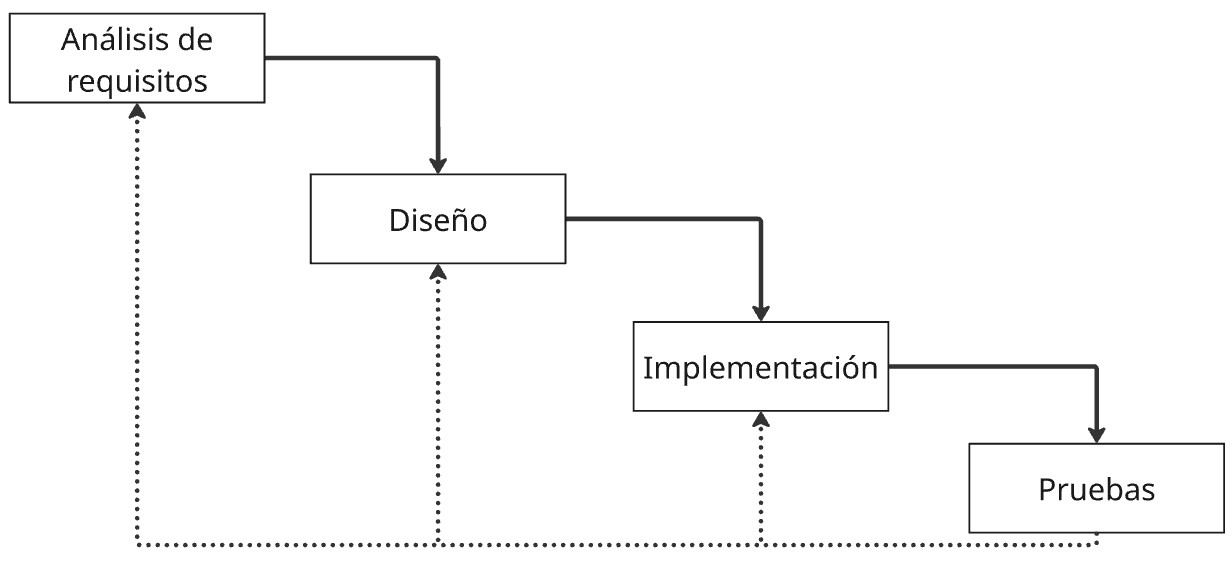
\includegraphics[width=0.8\linewidth]{img/modelo_cascada.jpg}
    \caption[Modelo en cascada realimentado.]{Modelo en cascada con realimentación. Las flechas continuas representan el flujo principal del proceso en cascada, mientras que las flechas punteadas indican las fases de realimentación.}\label{fig:modelo_cascada}
\end{figure}

El proyecto se organiza en las siguientes fases del ciclo de vida:

\begin{itemize}
    \item Análisis de requisitos: Consiste en las reuniones iniciales con los clientes, en este caso los directores del TFG. Se realiza un estudio de la bibliografía existente, se establecen los objetivos del trabajo y se traza un camino claro de los resultados que se quieren alcanzar.
    \item Diseño: Consiste en la investigación y selección de técnicas aplicables a la resolución del problema, incluyendo los conjuntos de datos y modelos a utilizar. En este apartado también se incluyen diversas pruebas preliminares y el diseño del software utilizado en la experimentación.
    \item Implementación: Consiste en la adaptación del código de los modelos investigados en la fase anterior, así como la implementación de nuevas funcionalidades.
    \item Pruebas: Consiste en la realización de diversos experimentos utilizando los conjuntos de datos y modelos previamente definidos. En esta fase se contempló (y efectivamente se llevó a cabo) la posibilidad de regresar a la fase de diseño, ya que, aunque algunos experimentos se definen inicialmente, la experimentación puede revelar nuevas posibilidades que deben ser evaluadas.
\end{itemize}

Además, de manera paralela a las etapas descritas anteriormente, se lleva a cabo un proceso continuo de redacción y documentación de la memoria del proyecto, en el que se formalizan todas las notas e investigaciones realizadas para cada capítulo, así como el detalle de cada decisión tomada durante el desarrollo del proyecto.

\begin{table}[h]
    \centering
    \small 
    \resizebox{\textwidth}{!}{ 
    \begin{NiceTabular}{c c c c c c c c c c c c c c c c c c c c c c c}[hvlines,color-inside]
        \Block[fill={cyan!50}]{2-1}{\textbf{Tareas}} & \Block[fill={cyan!50}]{2-1}{\shortstack{\textbf{Semanas - } \\ \textbf{Horas}}} 
        & \Block[fill={cyan!50}]{1-2}{\textbf{Enero}} &
        & \Block[fill={cyan!50}]{1-4}{\textbf{Febrero}} & & & 
        & \Block[fill={cyan!50}]{1-5}{\textbf{Marzo}} & & & &
        & \Block[fill={cyan!50}]{1-4}{\textbf{Abril}} & & &
        & \Block[fill={cyan!50}]{1-4}{\textbf{Mayo}} & & &
        & \Block[fill={cyan!50}]{1-2}{\textbf{Junio}} & \\ 
        
        & & \cellcolor{cyan!50} 20 & \cellcolor{cyan!50} 27 
        & \cellcolor{cyan!50} 03 & \cellcolor{cyan!50} 10 & \cellcolor{cyan!50} 17 & \cellcolor{cyan!50} 24 
        & \cellcolor{cyan!50} 03 & \cellcolor{cyan!50} 10 & \cellcolor{cyan!50} 17 & \cellcolor{cyan!50} 24 & \cellcolor{cyan!50} 31 
        & \cellcolor{cyan!50} 07 & \cellcolor{cyan!50} 14 & \cellcolor{cyan!50} 21 & \cellcolor{cyan!50} 28 
        & \cellcolor{cyan!50} 05 & \cellcolor{cyan!50} 12 & \cellcolor{cyan!50} 19 & \cellcolor{cyan!50} 26 
        & \cellcolor{cyan!50} 02 & \cellcolor{cyan!50} 09 \\
        
        Analisis de requisitos & $5 - 150$ & \Block[fill={gray!50}]{1-5} \\ 
        \\ 
        \hline
        Diseño & $4 - 120$ & & & & & & \Block[fill={gray!50}]{1-4} \\
        \\ 
        \hline
        Implementación & $2 - 60$ & & & & & & & & & & \Block[fill={gray!50}]{1-2} \\
        \\ 
        \hline
        Pruebas & $9 - 270$ & & & & & & & & & & & & \Block[fill={gray!50}]{1-9} \\
        \\ 
        \hline
        Documentación & -- & & & & & \Block[fill={gray!50}]{1-16} \\
    \end{NiceTabular}
    }
    \caption[Planificación temporal inicial del proyecto.]{Planificación temporal inicial del proyecto. La documentación se desarrolla de forma transversal a lo largo de la duración del proyecto, en paralelo al resto de fases.}\label{tabla:gantt-inicial}
\end{table}

\begin{table}[h]
    \centering
    \small 
    \resizebox{\textwidth}{!}{ 
    \begin{NiceTabular}{c c c c c c c c c c c c c c c c c c c c c c c}[hvlines,color-inside]
        \Block[fill={cyan!50}]{2-1}{\textbf{Tareas}} & \Block[fill={cyan!50}]{2-1}{\shortstack{\textbf{Semanas - } \\ \textbf{Horas}}} 
        & \Block[fill={cyan!50}]{1-2}{\textbf{Enero}} &
        & \Block[fill={cyan!50}]{1-4}{\textbf{Febrero}} & & & 
        & \Block[fill={cyan!50}]{1-5}{\textbf{Marzo}} & & & &
        & \Block[fill={cyan!50}]{1-4}{\textbf{Abril}} & & &
        & \Block[fill={cyan!50}]{1-4}{\textbf{Mayo}} & & &
        & \Block[fill={cyan!50}]{1-2}{\textbf{Junio}} & \\ 
        
        & & \cellcolor{cyan!50} 20 & \cellcolor{cyan!50} 27 
        & \cellcolor{cyan!50} 03 & \cellcolor{cyan!50} 10 & \cellcolor{cyan!50} 17 & \cellcolor{cyan!50} 24 
        & \cellcolor{cyan!50} 03 & \cellcolor{cyan!50} 10 & \cellcolor{cyan!50} 17 & \cellcolor{cyan!50} 24 & \cellcolor{cyan!50} 31 
        & \cellcolor{cyan!50} 07 & \cellcolor{cyan!50} 14 & \cellcolor{cyan!50} 21 & \cellcolor{cyan!50} 28 
        & \cellcolor{cyan!50} 05 & \cellcolor{cyan!50} 12 & \cellcolor{cyan!50} 19 & \cellcolor{cyan!50} 26 
        & \cellcolor{cyan!50} 02 & \cellcolor{cyan!50} 09 \\
        
        Analisis de requisitos & $8 - 240$ & \Block[fill={gray!50}]{1-8} \\ 
        \\ 
        \hline
        Diseño & $4 - 120$ & & & & & & \Block[fill={gray!50}]{1-4} \\
        \\ 
        \hline
        Implementación & $2 - 60$ & & & & & & & & & & \Block[fill={gray!50}]{1-2} \\
        \\ 
        \hline
        Pruebas & $9 - 270$ & & & & & & & & & & & & \Block[fill={gray!50}]{1-9} \\
        \\ 
        \hline
        Documentación & -- & & & & & \Block[fill={gray!50}]{1-16} \\
    \end{NiceTabular}
    }
    \caption[Planificación temporal final del proyecto.]{Planificación temporal final del proyecto. La documentación se desarrolla de forma transversal a lo largo de la duración del proyecto, en paralelo al resto de fases.}\label{tabla:gantt-final}
\end{table}

La planificación inicial del proyecto se detalla en la Tabla~\ref{tabla:gantt-inicial}. No obstante, debido al carácter novedoso del trabajo y a los continuos avances por parte de la comunidad científica a lo largo de este año, la planificación inicial experimentó algunas modificaciones. Estos ajustes estuvieron motivados por nuevos descubrimientos que permitieron comprender el fenómeno con mayor claridad, lo que obligó a retroceder a la fase inicial del proyecto y prolongó su duración. De este modo, la planificación final del proyecto se presenta en la Tabla~\ref{tabla:gantt-final}, mientras que en la Tabla~\ref{tabla:resumen-duracion} se presenta un resumen de la duración total.

\begin{table}[h]
    \centering
    \begin{NiceTabular}{l l}[hvlines,color-inside]
        \Block[fill={cyan!50}]{1-1}{Fecha de inicio} & $20$/$01$/$2025$ \\
        \Block[fill={cyan!50}]{1-1}{Fecha de fin} & $02$/$05$/$2025$ \\
        \Block[fill={cyan!50}]{1-1}{Duración} & $133$ días, $95$ laborables \\
    \end{NiceTabular}
    \caption{Resumen de las fechas de inicio y fin del proyecto, junto con la duración total.}\label{tabla:resumen-duracion}
\end{table}

Para la estimación del coste, partimos de la base de que el coste por hora de un investigador senior o responsable de I$+$D en una empresa tecnológica española es de $15$\euro/hora, según el portal de transparencia empresarial Glassdoor\footnote{Se asume un salario anual de $30000$\euro\ según estimaciones publicadas en: \url{https://www.glassdoor.es/Sueldos/ingeniero-de-investigacion-y-desarrollo-sueldo-SRCH_KO0,39.htm}}, y de una duración final del proyecto de $690$ horas. A esta cifra se deben sumar los gastos derivados de los distintos materiales utilizados, tales como el coste del portátil empleado en el desarrollo del TFG y el uso de un servidor GPU de altas prestaciones, junto a otros gastos misceláneos entre los que se incluye el consumo eléctrico. El desglose detallado de estos costes se puede consultar en la Tabla~\ref{tabla:estimacion-coste}.

Respecto al servidor GPU, y basándonos en sus especificaciones, se estima su valoración en $12000$\euro. Se asume una amortización proyectada a lo largo de dos años, lo que equivale a un coste diario de $16.44$\euro. Por ende, la contribución total de este servidor al coste del proyecto sería de $2186.52$\euro.

\begin{table}[h]
    \centering
    \begin{tabular}{|l|>{\raggedright\arraybackslash}p{2in}|} 
        \hline
        \cellcolor{cyan!50} \hspace{6em} \textbf{Item} & \cellcolor{cyan!50} \hspace{4.5em} \textbf{Costo} \\ 
        \hline
        Salario & 10 350.00\euro \\
        \hline
        Portátil de Gama Media & 1 000.00\euro \\
        \hline
        Servidor GPU & 2 186.52\euro \\
        \hline
        Otros & 300.00\euro \\
        \hline
        \cellcolor{cyan!50} \hspace{12em} \textbf{Total} & 13 836.52\euro\\
        \hline
    \end{tabular}
    \caption{Estimación del coste del proyecto.}\label{tabla:estimacion-coste}
\end{table}

\endinput
